\documentclass[10pt,a4paper,oneside]{article} %report expects chapters?

% http://en.wikibooks.org/wiki/LaTeX/Page_Layout
%\pdfpagewidth = 441 % 441x666 
%\pdfpageheight = 666

\usepackage[latin1]{inputenc}   % St�tte for direkte input av norske tegn
\usepackage{graphicx} % for \includegraphics
\usepackage{hyperref} % for click-able TOC links and \cite's in PDF
\usepackage{float}
\usepackage{mathtools}
\usepackage{fancyvrb}
\DeclareRobustCommand{\orderof}{\ensuremath{\mathcal{O}}}
\usepackage{xfrac} %for slantfrac a.k.a. sfrac
\begin{document}

\setcounter{page}{-100}
\pagestyle{empty} % no page numbers
\begin{titlepage}

\emph{Rendering based on hybrid methods}

by Torbj�rn Haugen and P�l Solberg Trefall
\today

\begin{figure}[htbp]
	\centering
		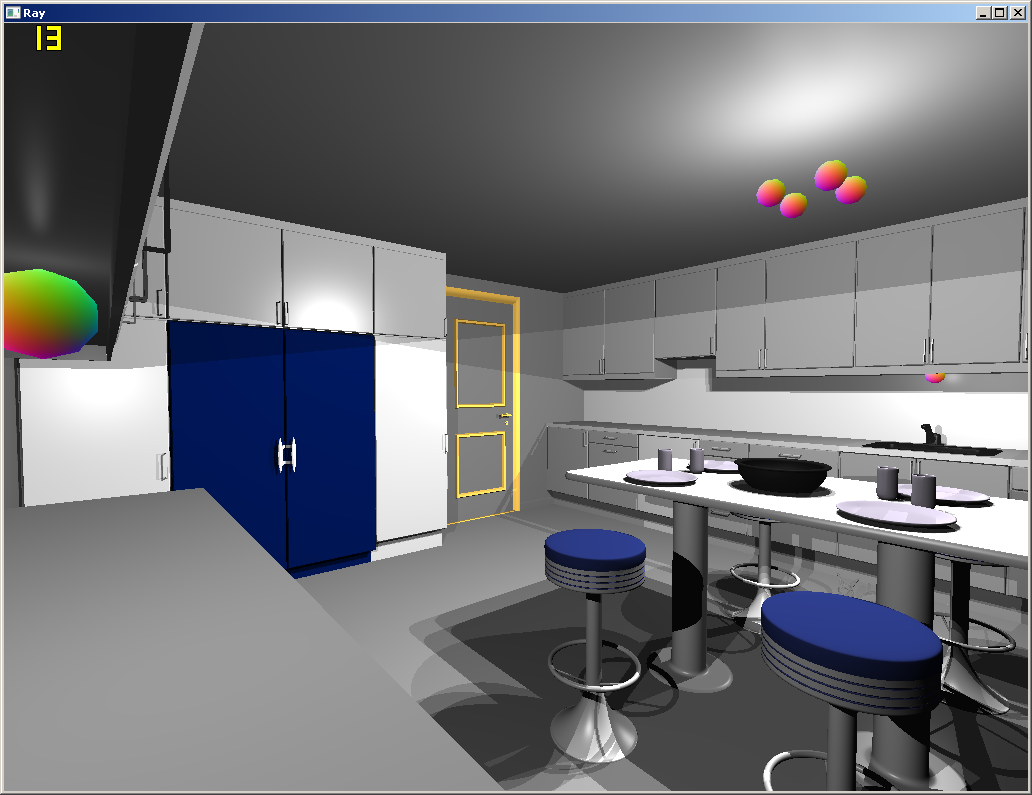
\includegraphics[width=0.90\textwidth]{0/all_lights.png}
	\caption{BART Kitchen}
	\label{fig:all_lights}
\end{figure}

\end{titlepage}
\setcounter{page}{-99}

\begin{abstract}
We are going to study various rendering techniques, and compare them to a renderer that combines deferred shading and raytracing.
\end{abstract}
\pagestyle{plain} % turn page numbers on
\setcounter{page}{0}

\tableofcontents


\begin{abstract}
We are going to study various rendering techniques, and compare them to a renderer that combines deferred shading and raytracing.
\end{abstract}
\part{Previous work}

There are few commercial rendering engines that combine rasterization and raytracing. Virtually all computer games use rasterization. The demand for graphical fidelidy has driven the development of programmable GPUs. For some time now, it has been possible to implement direct/Whitted-style and pathtracing on a GPU.

Exampels of real time direct raytracing engines. Manta, Razor, Arauna.
Examples of real time path tracing engines. SmallPT, Brigade.

Examples of hybrid engines; Pixar's REYES

\paragraph{Hybrid shadows} renders world space positions to a texture. Texture is loaded into optix, from there a ray is traced from each world space position against all lights. Attenuates given world space position and saves attenuation value in a shadowmap.

\paragraph{ISG Shadows} Image Space Gathering \cite{nvidiarobison09}
\paragraph{ISG Reflection}


\section {Global Illumination (GI) techniques}
	\subsection{Pure raytracing} 
		One pass. But produces ugly hard shadows unless we shoot more that one shadowray.
	\subsection{Photon mapping} A two pass algorithm. Combines ray tracing and particle tracing.
		\paragraph{1.st pass} photons are cast from the light source and checkt for intersection against the scene.    Every intersecting photon is stored in a photon map. After intersecting the scene a photon may be reflected, refracted or absorbed depending on the material properties of the surface. The selection is done by the Monte Carlo method called 'russian roulette'. If the photon is not absorbed, then a new traveling direction is calculated for it according to the selected behavior.
			
		\paragraph{2.nd pass} View rays are cast from the camera and checked for intersection against the scene similar to raytracing. Once the nearest intersection point is found, a pre-defined number of nearest photons are sampled, and interpolated to calculate irradiance at that point.

	\subsection {Radiosity}
		Diffuse inter-reflections of light in a scene. Divides scene geometry into small
		patches. For every pair of patches, one defines a camera model for how they can
		see each other. Ex: paraboloid, cuboid-mapping. These form factors are then used
		in an iterative process that progressively transfers radiation between the
		patches.

		Can generate realistic diffuse lighting and is viewpoint independant. As long as
		geometry and lightsources remain unchanged, the simulation can be effectively
		sotred and sampled to obtain the scene lighting for any view.

		Con: Limited diffuse lighting effects. Can't do absorb, refract?

	\subsection {Instant Radiosity}
		A technique developed by Alexander Keller to approximate the simulation of light
		transfers between purely diffuse surfaces. The algorithm goes as follows, first
		one casts a large quantity of rays from each light in random directions which
		are then checked for intersection against the scene. Then, at the intersection
		point create a so called 'virtual point light' (VPL). These VPLs represent the
		light bouncing off surfaces. Accuracy may be improved by recursively casting new
		light rays from each VPL, but one step usually creates a reliable approximation.
		Once the VPLs have been created, they are rendered as normal point lights.
		Modern GPUs are very good at this.

	\subsection {Path Tracing}
		Path tracing combines ray tracing and Monte Carlo methods to approximate the
		integral of incoming light at each point. It is one of the most physically
		accurate methods, but also one of the most demanding ones in terms of
		computations. Path tracing is naturally capable of generating effects like depth
		of field, caustics and soft shadows. The idea is to cast many rays at each
		intersection. The number of rays is decided by the properties of the intersected
		surface, for example its BRDF. If we as an example take a diffuse surface, then
		rays are distributed on the hemisphere above the intersection point. But, if the
		surface is glossy, then the generated rays are distributed around the reflection
		vector. There are many methods that improve the performance of this brute force
		method, such as stratified sampling, importance sampling and a modification
		called 'Bidirectional Path Tracing' that is useful to increase the chance of a
		ray intersecting a surface in scenes with small or occluded light sources.

\section {Real-time Global Illumination}
	Recent advancements were made by taking classical algorithms and implementing
	them on GPUs. These effects have been adapted to rasterization, examples are:
	ambient occlusion, soft shadows, depth-of-field, atmospheric scattering and water reflections and refractions.

	\subsection {Screen Space Ambient Occlusion}
		Screen Space Ambient Occlusion (SSAO) is a technique that was recently pioneered by Crytek. It approximates ambient occlusion in real-time on the gpu. The technique is decoupled from the scene complexity and requires a smaller amount of rays than the original ambient occlusion technique. It relies entirely on the depth buffer, this means geometry outside whats visible can not cause occlusion.

	\subsection {Screen Space Global Illumination}
        Screen Space Global Illumination (SSGI) is an extension of SSAO that generates a rough approximation of global illumination on a small scale. SSGI works by sampling colors from the rendered image of the scene to simulate secondary light bounces, it there for suffers from the same limitations as SSAO, so it can only show light interactions between objects that are very close to each other. Despite these limitation it is useful when combined with a coarse global illumination technique like instant radiosity. This way, SSGI can provide high-frequency global illumination and instant radiosity provides coarse, low-frequency global illumination.

	\subsection {Image Space Photon Mapping}
		The photon mapping algorithm has been adapted for real-time use in an algorithm called image space photon mapping (ISPM), that generates the information about the first bounce of photons on the GPU using Reflective Shadow Maps (RSM). \cite{dachsbacher2005} 
		From this initial distribution of photons, a reduced set is selected and recursively raytraced on the CPU similarily to original photon mapping. The consecutive bouncing of each photon is stored and sent back to the GPU for rendering. On the GPU, the photons are used to estimate lighting using a scattering approach, the opposite of the gathering approach used by classical photon mapping. The scattering is performed by rendering ellipsoid-shaped volumes in screen space that represent the influence of each photon on the pixels around it. For each pixel affected by the photon volume, the scene properties are sampled and the lighting contribution of that photon is computed for that pixel. ISPM is capable of mathematically identical results to traditional photon mapping as long as it is rendered at full screen resolution.

		\begin{figure}
			\centering
				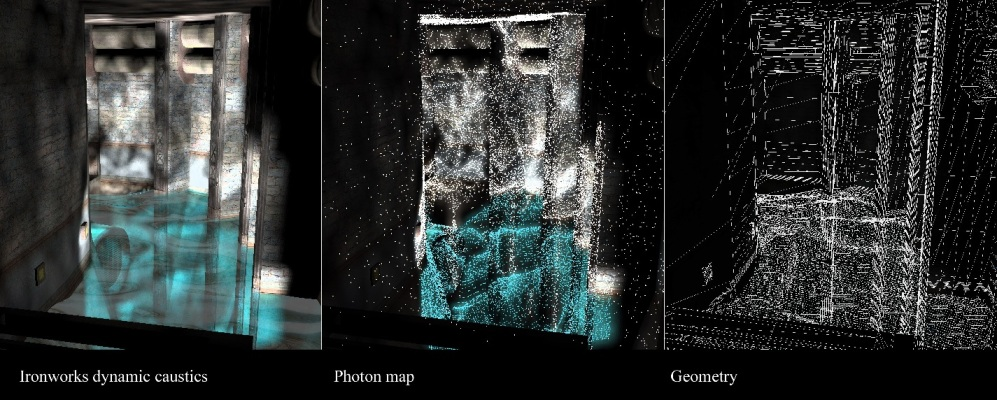
\includegraphics[width=1.00\textwidth]{previous_work/ispm.jpg}
			\caption{McGuire and Luebke's ISPM extension}
			\label{fig:ispm}
		\end{figure}

	\subsection {Global Illumination with Light Propagation Volumes}

	Global Illumination with Light Propagation Volumes (LPV) is a technique for approximation instant radiosity on the GPU. \cite{kaplanyan2009} This technique avoids the instant radiosity requirements for processing a large amount of lights by using a representation of the scene lighting that decouples scene illumination from light quantity. The first step is to generate an initial distribution of VPLs, this is done by rendering a Reflective Shadow Map (RSM) \cite{dachsbacher2005} from the lights point of view. The radiance of each VPL is injected as spherical harmonics into a 3D texture as spherical harmonics that represents the initial distribution of radiance on the scene. Then the initial radiances are propagated iteratively through the radiance volume to simulate light propagation. The volume is then sampled once per-pixel to obtain the irradiance at that location.

\subsection {Real-Time Ray Tracing}
	Inigo Wald. SIMD. packet tracing. openRT. 
	\paragraph{Arauna} uses kd-tree for static. bih for dynamic.

\subsection {Real-Time Path Tracing}
	One of the most complex global illumination algorithms. 
	\paragraph {Nvidia Optix} demonstration
	\paragraph {Brigade} 
	\paragraph {V-ray}

\subsection {Combining Rasterization and Ray Tracing}

Rasterization and Ray Tracing are very different, but can be combined to exploit each ones strengths. Rasterization is good at direct lighting, while raytracing is flexible for many effects.

\subsubsection {RenderMan}

By Pixar.

% part c
% chapter % funker ikke for article virker det som section subsection
% subsubsection 
% paragraph 
% subparagraph

\part{Rasterizer}


\section{Introduction}
Rasterization is an object order method. We have a list of objects in our scene and draw one after another. This is the opposite of an image order rendering technique, like raytracing, where each pixel is traversed. This is why raytracing can be slower than rasterization; -testing each pixel and, for each pixel, testing every object. This pipeline can require more computation than a rasterization pipeline, which is iterating over every object once and coloring the pixels the object occupies.

Raytracing can be accelerated by spatial sorting, like bounding volume hierarchies, but so can rasterization. Frustrum- and occlusion-culling are just two examples.

The most basic job of a rasterizer is to draw triangles using pixels on a raster display. A popular method is scanline rendering, because of cache locality and the way displays update their image a scanline at a time.

\begin{figure}[H]
  \centering
  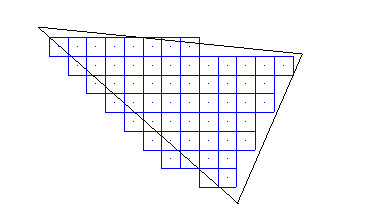
\includegraphics{Media/raster_scanline.png}
  \caption{Scanline rasterization of pixels}   
  \label{fig:Scanline rasterization of pixels}
\end{figure}


\section{Rasterization Pipelines}

Write something general about rasterization pipelines, to introduce the concept.


\subsection{Forward Rendering}

\begin{figure}[H]
	\begin{math}
		\orderof(\sum {pixel_{rasterized + shaded}} \times \sum light)
	\end{math}
	\caption{The rasterization and shading complexity of a Forward Rendering Pipeline}
	\label{fig:FRP_complexity}
\end{figure}

In a forward rendering pipeline (FRP), all surfaces are shaded immediately. As figure~\ref{fig:FRP_complexity} show, this doesn't scale well as the number of lights go up.

\subsubsection{Multiple Lights}

There are different methods for dealing with multiple lights in an FRP. These different approaches all have their strengths and weaknesses.

\paragraph{Ubershader}

The Ubershader is a single-pass shader that handles any material and light combination or programatically create different shaders for all material- and light-type combinations. Creating an uber-shader becomes unwieldy as the types of lights and materials increase due to combinatorial explosion, each material-light pair will require custom code.

\paragraph{Multi-pass}

Another way of shading a surface with an arbitrary number lights is using a multi-pass technique. Each geometry is shaded with each light at a time. The framebuffer is set to blend fragments together, combining the effect of each light. Multi-pass rendering requires re-drawing the entire mesh for each light and requires transforming vertices and rasterizing each pass, making the scene quickly vertex and fillrate bound.

\subsection{Deferred Rendering}

\begin{figure}[H]
	\begin{math}
		\orderof(\sum {pixel_{rasterized}}) + \orderof(\sum {pixel_{GBuffer}} \times \sum {light})
	\end{math}
	\caption{The rasterization and shading complexity of a Deferred Rendering Pipeline}
	\label{fig:DRP_complexity}
\end{figure}

Deferred Rendering Deering1988 is a rasterization-based rendering technique in which the result of drawing the scene is divided and stored in intermediate buffers (called the G-Buffer) using multiple render targets (MRT).  The G-buffer, or Geometry-Buffer, is called so because it stores per pixel geometric properties like depth, normals and texture coordinates; - a caching of the geometry that the camera is viewing, for repeated use further down the rendering pipeline. The G-Buffer is input into a shading algorithm, usually as samplers, to produce the final result. This reduces the input of the scene to what is in the view space when performing shading, and specially reduce the cost of lighting. Lights are rendered in a second pass as geometric volumes, who's surface color is accumulated into a final render target using additive blending. In essence, this gives us a rendering pipeline which drives a single pass per light, as opposed to forward rendering's single pass with a complex shader or multi-pass techniques (typically single pass per mesh per light).

Historically, deferred rendering has had some limitations. Due to the nature of the G-Buffer, transparency couldn't be supported directly in the deferred pipeline. Instead, a forward renderer has commonly been used for handling transparent objects in the scene. Further, a deferred pipeline can't take advantage of Multisample anti-aliasing (MSAA) in hardware, forcing quite expensive anti-aliasing filters to be programmed into the pipeline. The amount of parameters one can pass to shader programs is also directly limited by the size of the G-Buffer, and the amount of render targets supported. This forces a deferred pipeline to be quite expensive, bandwidth and memory wise. Further, due to how a deferred pipeline accumulates the color of lights using additive blending, overlapping lights cause overhead.

On the positive side, a deferred rendering pipeline is greatly simplified and more general than a forward rendering pipeline. The scene is rendered with one shader program, filling the G-Buffer, and then the G-Buffer is handled in multiple passes by different shader programs, like the lighting pass, shadow pass, and so forth. These shader programs can also be simplified, as everything in the G-Buffer used for the shading, already is in screen-space. The cost for light calculation is greatly reduced compared to a forward renderer, since shading is only done in screen-space for geometry that is visible by the camera; there is no wasted shading effort.

A deferred shading approach could lend well as a hybrid foundation of rasterization and raytracing, as the G-Buffer data could be generated by any method, as long as it is in screenspace, and could also be used as a first-ray lookup for a raytracer.

Over the years, multiple improvements to the deferred rendering approach has been applied in practise. Light pre-pass, tile-based deferred rendering and decoupled deferred rendering are listed among the most popular and more recent approaches.

\subsubsection{Light pre-pass}

Light pre-pass was first presented by Wolfgang Engel [Engel2008]. In this approach one would in a first pass render geometry information into a G-Buffer that is required for light-calculation, like depth, normals and specular power. In a second pass one would render the light geometry into a render-target using the G-Buffer for information about the scene. In a third pass, one would use normal forward-rendering, but use the light render target as sampler for the lighting, thus getting the reduced cost of lighting from a deferred rendering pipeline, while retaining much of the strengths and flexibility of a forward rendering pipeline. 

This forces three passes to render the scene, although each pass is cheaper than in a pure deferred pipeline, and consume less bandwidth and memory than the deferred pipeline. Using light pre-pass, one can even prevent usage of MRT. In essence, using this approach we end up with a pipeline which is single pass per mesh.

Looking at the limitations of light pre-pass, it still doesn't solve the problem with transparency in a deferred pipeline. Also, it is limited in variety of lighting due to the lighting buffer, and if sticking with a four-channel buffer for lights, both colored specular and more advanced shading models, like Oren-Nayar, isn't easy to achieve (although there are solutions to be found [BlindRenderer2011]). Further, the flexibility in the material properties of the third pass of the light pre-pass pipeline is illusive. One would think that the forward rendering nature of this pass would grant great flexibility in the property input to the shader program for each mesh, but what largely defines a material, is how its surface interacts with light. Thus, the limitations of the lighting buffer directly limits the flexibility of material properties.

On the positive side, we get hardware MSAA for the third geometry pass, even though the lighting buffer doesn't get this hardware anti-aliasing treatment.

\subsubsection{Tile-based Deferred Rendering}

A tile-based deferred rendering pipeline divides the screen space into tiles, the goal being to map which tiles each light intersects and thus greatly reduce the number of pixels to process for shading per light, and reduce the overhead of overlapping lights. In [Andersson2009], it's pointed out how the light-classification per screen-space tile is similar to how Compute Shaders can work with 2D thread-groups; - this is a case that should be convertible to other GPU compute APIs like OpenCL and Cuda. 

Using a computing API, the G-Buffer and depth is read only once, minimizing bandwidth, where a pure shader-based solution would have to multiple reads. All lighting is resolved with gpgpu before the shading result is finally written out to a buffer immediately available to the shader pipeline. Thus we don't need an intermediate light buffer, as with light pre-pass, and it scales much better with overlapping lights due to the fine-grained culling in tiles (eg. 16x16 tiles).
\section{Raytracing}

\subsection{Introduction}
OptiX is a closed source raytracing engine designed by Nvidia, and currently only works on their own GPUs. The library is free to use both for hobbyists and for commerce. One can speculate that it will be opened up further once equivalent vendor agnostic libraries become available.

Optix can be seen as a framework for launching rays. It doesn't know anything about lights, shadows, ambient occlusion or any other rendering detail for that matter. What it does know is; rays, how to build and traverse acceleration structures, geometry representation and how to traverse the scene.What makes OptiX interesting is programmability; a variety of ray tracing-based algorithms in graphics and non-graphics domains can be implemented \cite{Parker10OptiX} by creating custom programs.

\subsection{Programs}
\paragraph{There are eight} different types of user provided programs in OptiX. These programs are implemented using the CUDA C-language. They all operate on a single ray at a time, except for the bounds program, which is used to determine bounds for acceleration structure construction. For triangle geometry, Optix can access individual vertices of a mesh for constructing a k-dimensional-tree (kdtree) or split bounding volume hierarchy  (sbvh).

\begin{enumerate}
	\item {
	\textbf{Ray generation}
      programs (``raygen'' from here on) are launched by the client program using rtContextLaunch(rayProgramIndex, with, height). This invokes many raygen programs in parallel. The raygen is the main entry point into the raytracing pipeline. Input and output buffers are declared inside. You can use a single raygen program as a general compute shader, but the intended use is to implement a camera model by initializing ray origin and direction. After a ray has been initialized, \begin{verbatim}rtTrace startNode,ray,payload \end{verbatim} can be called, and will trace all of start nodes children. 
	}

	\item{\textbf{Exeption} programs are invoked when the system encounters problems like out of stack space, or buffer access index is                   out of range. Also supports user-defined exceptions that can be 	thrown from any program. Can react by printing                         diagnostic messages or   writing specific color values to an output buffer.}

	\item{\textbf{Closest hit} programs are invoked once traversal has found the closest intersection of a ray with scene geometry.}

	\item{\textbf{Any hit}
		allow shading to be kept separate from geometry.
		May call rtTerminateRay and stop all traversal. Early ray termination for shadowrays and AO.
		Also useful for binary transparency by texture look up.
		Default any hit program is a no-op, often the most desired operation.
		}

	\item{\textbf{Miss} intersect any geometry. }

	\item {\textbf{Intersection}
	programs are needed to describe geometry. The program must at least report if and where the ray touches the object, 
	additional computations may involve normals, texture coordinates and other attributes based on hit position.
	Intersection programs allow you to trace perfect spheres, cylinders, cubes,  CSG-surfaces, parametric surfaces like
	Bezier and NURBS, fractals and of course triangle meshes. Parker \cite{Parker10OptiX} notes \begin{quote} programmable intersection op-
	eration facilitates direct access to the native format, which can help
	avoid copies when interoperating with rasterization-based systems.\end{quote} In our program we store vertex attributes continuously (first all positions, then all normals, etc.) as opposed to storing them interleaved (one position, one normal and so on). Unfortunately, the built in acceleration sbvh and kdtree builders expect triangle geometry to be interleaved, so we settled for the generic bvh builder.
	}
	
	\item{\textbf{Selector}
		visit programs gives on control over graph traversal.
		The program can do traversals based on data stored in a visitor programs payload and make a traversal decision based 	on that data.
	}

 \item{\textbf{Bounding box}
		programs obviously compute the bounds associated with each primitive to enable acceleration structures over any geometry. The bounding box program takes a primtive index and computes its bounds. From the client api, a node is associated a given bounds program.
	}
 				
\end{enumerate}

The closest hit, any hit and miss programs determine shading. The raygen, selector and intersection programs determine scene traversal.
			 
\subsection{Client-side API}

To begin raytracing a scene ``rtContextLaunch( raygenIdx, width, height )'' is called with a given Rey Generation Program index as a parameter. From the ray generation program ``rtTrace( rootNode, ray, payload )'' is given the root scene node for traversal. During traversal, if a node a nodes associated selector and acceleration program is run.
If the acceleration traverser determines that a primitive node is hit, it invokes the primitives intersection program.
If the Intersection program calls ``rtReportIntersection'', the primitives associated ``material'' Any Hit Program is called.
If the ray doesn't hit anything, a miss program is called. The missprogram is always required.

\subsection{CUDA program API}

\paragraph{A simple raygen program:}

\begin{verbatim}
// notice use of templates for type and dimension
rtBuffer<unsigned char, 2> outputBuffer; 

RT_PROGRAM void pinhole_camera() {
  Ray ray = PinholeCamera::makeRay( launchIndex );
  UserPayload payload;
  rtTrace( topObject, ray, payload );
  outputBuffer[launchIndex] = payload.result;
}
\end{verbatim}


\part{Hybridity}
\section{Why Hybrid}

Virtually all optical phenomena can be modelled using ray tracing. The same can not be said for rasterization. 

\subsection{Rendering effects that are tricky using rasterization}

	\paragraph A typical problem with rasterization is the blending order of fragments needed for translucent surfaces. This is required if a scene contains more than one planar glass surface or any curved glass. Blending order can be solved using an A-buffer \cite{carpenter_1984} at the cost of program complexity and memory. 

	\paragraph Shadows using shadow maps have many problems. Ray tracing dosn't suffer aliasing to the same extent.

	\paragraph Reflections must be done by rendering the scene seen from the surface that is to recieve reflections. Usually the scene is rendered into a cube map using six cameras. This is a crude approximation. Creating multiple reflection bounces quickly becomes more expensive. All surfaces visible in the reflection must be rendered multiple times. A ray tracer in comparison only needs traverse the rays affected.

	So, will we in the future, once computational power is good enough to raytrace at retinal display quality only use ray tracing? Probably not. We surround ourselves with objects that essentially only have diffuse shading. Glass house and porcelain shops are the exception, and even in such scenes, there are an abundance of diffuse surfaces.

	Raytracing is essential for reflections. Just look at this car:

	\begin{figure}[ht]
		\centering
		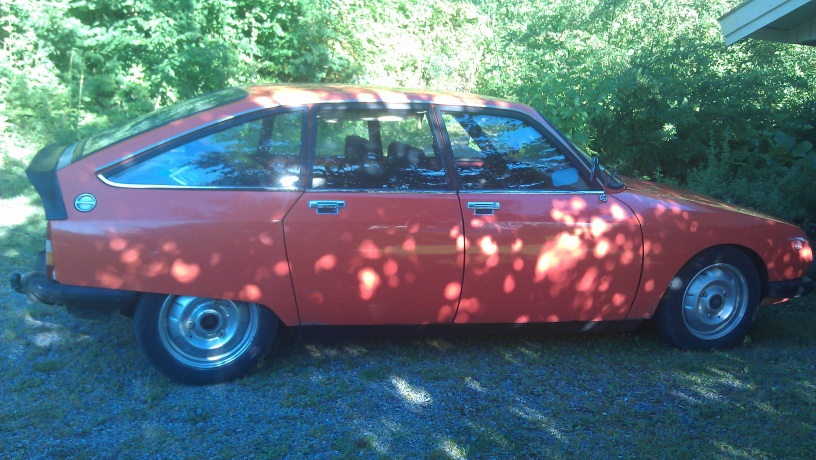
\includegraphics[width=0.80\textwidth]{Media/why_hybrid_carphoto.jpg}
		\caption{The car paint, glass and chrome details are essentially the only reflective surfaces in the scene}
		\label{fig:citroen_gs}
	\end{figure}
	
	\paragraph{Fill(rate) workload}
	With rasterization, we often tell the GPU to shade large surfaces that's out of view, the GPU quickly clips and discards fragments out side the view frustum. Pixar, as mentioned earlier solves this by cutting the geometry until it fits.

	Ray tracing doesn't have this problem. We only try to shade what is visible.

	\paragraph For a raster to be able to render anything, it must be converted to triangles. There are types of geometry where it may be more efficient in both terms of speed and memory to use a raytracer.

	Some examples are:
	\begin{itemize}
		\item Distance Fields can be raymarched, or an iso value can be extracted by solving the fields equation in an analytic raytracer. A rasterizer must usually sample all of the         field inside the view volume. This becomes especially problematic if the field changes on a frame-by-frame basis.

		\item Scalar Volume Data. Instead of rendering slices or iso-surfaces, the raw data can be sampled using discrete raytracing (also known as ray marching). %cite [Kajiya1986] The rendering equation ???

		\item Spline surfaces
		\item Perfect analytical surfaces
	\end{itemize}

\subsection{Reasons to use a hybrid}

Its the future. Hardware is becoming increasingly parallel. Ray tracing is trivially parallellizable. Ray tracing won't replace rasterization over night, but it will become increasingly useful.

Its conceptually simpler. Shaders can be written with fewer dependencies. Trading memory and programmer time for compute power.

As mentioned, certain types of geometry are better suited for ray tracing.

	\begin{figure}[ht]
		\centering
		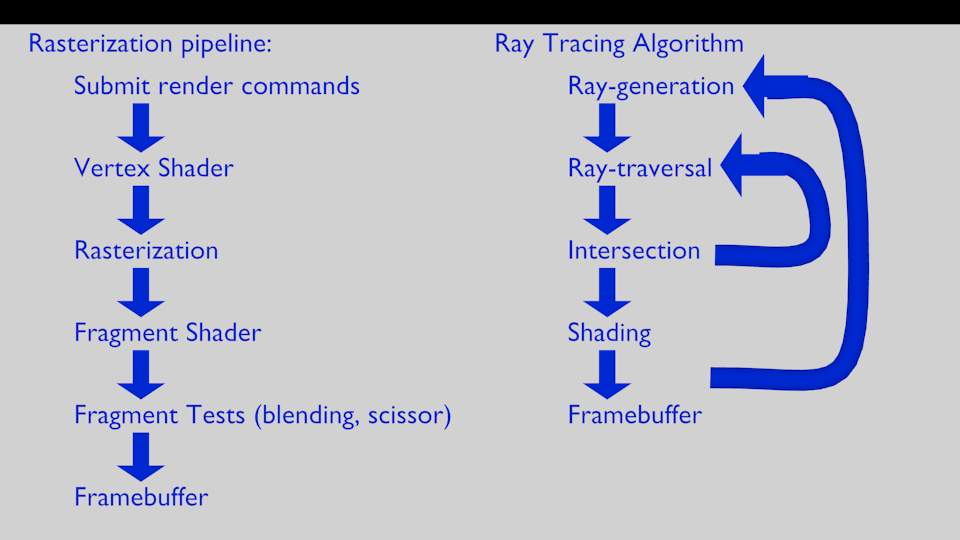
\includegraphics[width=0.80\textwidth]{Media/why_hybrid_pipeline_diffs.png}
		\caption{Rasterization can be done in one pass, while ray tracing is recursive}
		\label{fig:pipelines}
	\end{figure}

Rasterization has recieved a lot of attention due to its efficiency. This efficiency is mainly due to its cache and bandwidth friendliness. Notice in the figure \ref{fig:pipelines} comparing rasterization pipeline and ray tracing algorithm that rasterization has a predictable flow from one stage to the next, while ray tracing has arrows that signify recursive calls for continued traversal, or recursive materials when shading. Unless someone invents memory with bandwidth on par with CPU registers, ray tracing will allways be slower.

	\begin{figure}[ht]
		\centering 
\includegraphics[width=0.80\textwidth]{Media/why_hybrid_raymindmap.png}
		\caption{ray tracer strengths}
		\label{fig:ray_mmap}
	\end{figure}
	
	\begin{figure}[ht]
		\centering 
\includegraphics[width=0.80\textwidth]{Media/why_hybrid_rastermindmap.png}
		\caption{raster strengths}
		\label{fig:raster_mmap}
	\end{figure}

In a raytracer, global effects, such as reflections, refractions and shadows, are handled per fragment.

\section{OptiX and GL interopability}


Combining our deferred raster pipeline with OptiX can either be done from scratch, learning what every OptiX API-call does, or, copy one of the GL/Optix interop examples and modify it until it works. 

\subsection{Shared State}

The following state must be synchronized between GL and OptiX

\begin{enumerate}
	\item Geometry and its transform (model matrix)
	\item Textures (if we find that they can demonstrate any advantages)
	\item Camera (view matrix \& projection matrix)
\end{enumerate}

For geometry, ``optix::Context'' provides functions createBufferFromGLBO and similar createTextureSamplerFromGLImage for textures.

The standard pinhole\_camera.cu implementation is used, then the view vectors (u,v,w) must be extracted from our camera class or the modelview matrix.

\paragraph{Description of the rendering pipeline}

GL and OptiX scenes are independently rendered. We end up with two sets of g-buffers, shading and composition is done in a shader.


\section{Implementation}

\subsection{Engine architecture}
The architecture of the engine is mainly focused on the concepts of file loading and parsing, object oriented wrapping of OpenGL, scene objects, and render passes.

\subsubsection{File loading and parsing}
\paragraph{BART}
Write something about BART.
\paragraph{Assimp}
Write something about Assimp.
\paragraph{Shaders}
Write something about shader loading.
\paragraph{Textures}
Write something about texture loading.
\paragraph{Materials}
Write something about material loadaing and parsing
\paragraph{Configuration}
Write something about configuration loading and parsing.

\subsubsection{Object oriented OpenGL wrappers}
As was explained in chapter (about OpenGL), the OpenGL API is a stack-based state machine. In an engine architecture, it makes for more robust handling when a certain behavior is grouped or stored within a class, and take advantage of the construction of objects and destruction of objects, to automate the state of the OpenGL stack as much as possible.

\subsubsection{Scene objects}
The scene consist of multiple graphical objects positioned on the screen, and scene objects represents these by declaring the OpenGL render buffers, etc...

\subsubsection{Render pass}
A render pass defines a group of scene objects to be rendered by the rasterizer or raytracer, and can write to render buffers or the back buffer. The SceneManager object defines the order in which the different passes are called, and often one render pass depends on another in order to move down the render pipeline. For instance, the final light pass requires that at least the g-buffer pass has been made in order to work.

\subsection{Deferred pipeline}
The pipeline of the deferred renderer is broken up into two render passes. The G-buffer pass and the final light pass.

\subsubsection{G-buffer pass}
In the G-buffer pass, all geometry in the scene is rendered by the rasterizer. Position, diffuse and normal data is stored in an MRT in view space.

\subsubsection{Final light pass}
In the Final light pass, a fullscreen quad is rasterized. For each pixel on the screen, each light in the scene interact with what is stored in the G-buffer for that pixel. The result is written to the back-buffer and displayed on the screen.

\subsection{Camera model}
The raytracer uses pinhole camera model. The eye is a point, rays are cast from this point, through the viewplane and into the scene. Eyepoint-viewplane distance determines focal length. A rasterizer on the other hand requires a projection matrix.

\subsection{Various hybrid configurations}

\subsection{Geometry}
Traditional triangle meshes with vertex attributes (normals, texture coordinates etc)


\section{Results}


Write some results.


\part{Conclusion}

\section{Concluding remarks}
We have reviewed how rasterization and ray tracing techniques can be combined to make steps towards photo-realistic, real-time rendering. We identified that the deferred rendering pipeline was a good choice for the rasterization stages, since it easily allows the rasterized g-buffer data to be stored in view space. This is the same space that is output from a raytracer, and makes it simpler to mix the results from the two different rendering techniques.

\begin{figure}[H]
	\centering
	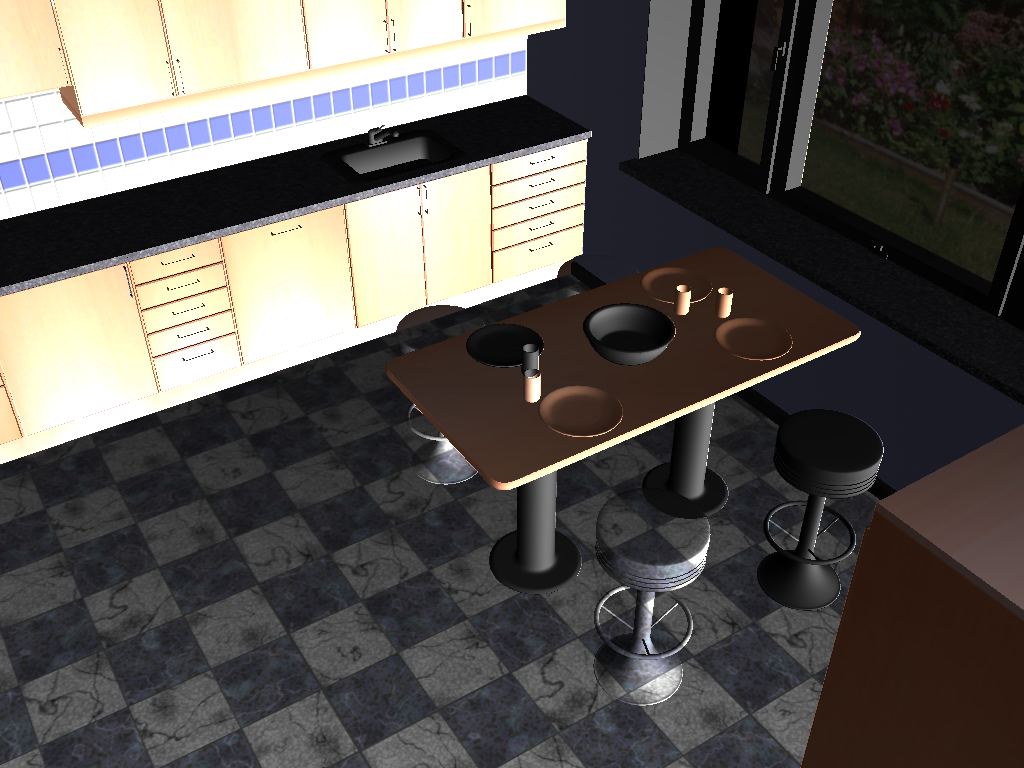
\includegraphics[width=1.00\textwidth]{Media/hybrid.png}
	\caption{Geometry rasterized, normals raytraced. Three of the chairs, and some of the dishes, were only raytraced.}
	\label{fig:hybrid_image01}
\end{figure}

The OptiX raytracer API was a good choice for the dissertation work, since it was a complete raytracer implemented on top of Cuda, with accelerated structure support and it's interopability based on Cuda's strong foundation.

In our Hybridity chapters, we identified several rendering problems where the raytracer would be stronger than a rasterizer. Order independent transparency, aliasing-free shadows, reflections and refractions, analytical geometry and volumetric data are a few.

Through our tests, we found that it's quite limited how large part of the scene, and which techniques, can be handled by the ray-tracer, and still keep within the scope of real-time framerates. Interopability alone eats a lot of time. Some tests using DirectX and Computer Shaders showed that the same algorithm would run up to a hundred percent faster than an OpenGL and Cuda interop equivalent. The OpenGL 4.3 specification, that introduce Compute Shader support to OpenGL, was released too late for us to take advantage of it in our work.

\begin{figure}[H]
	\centering
	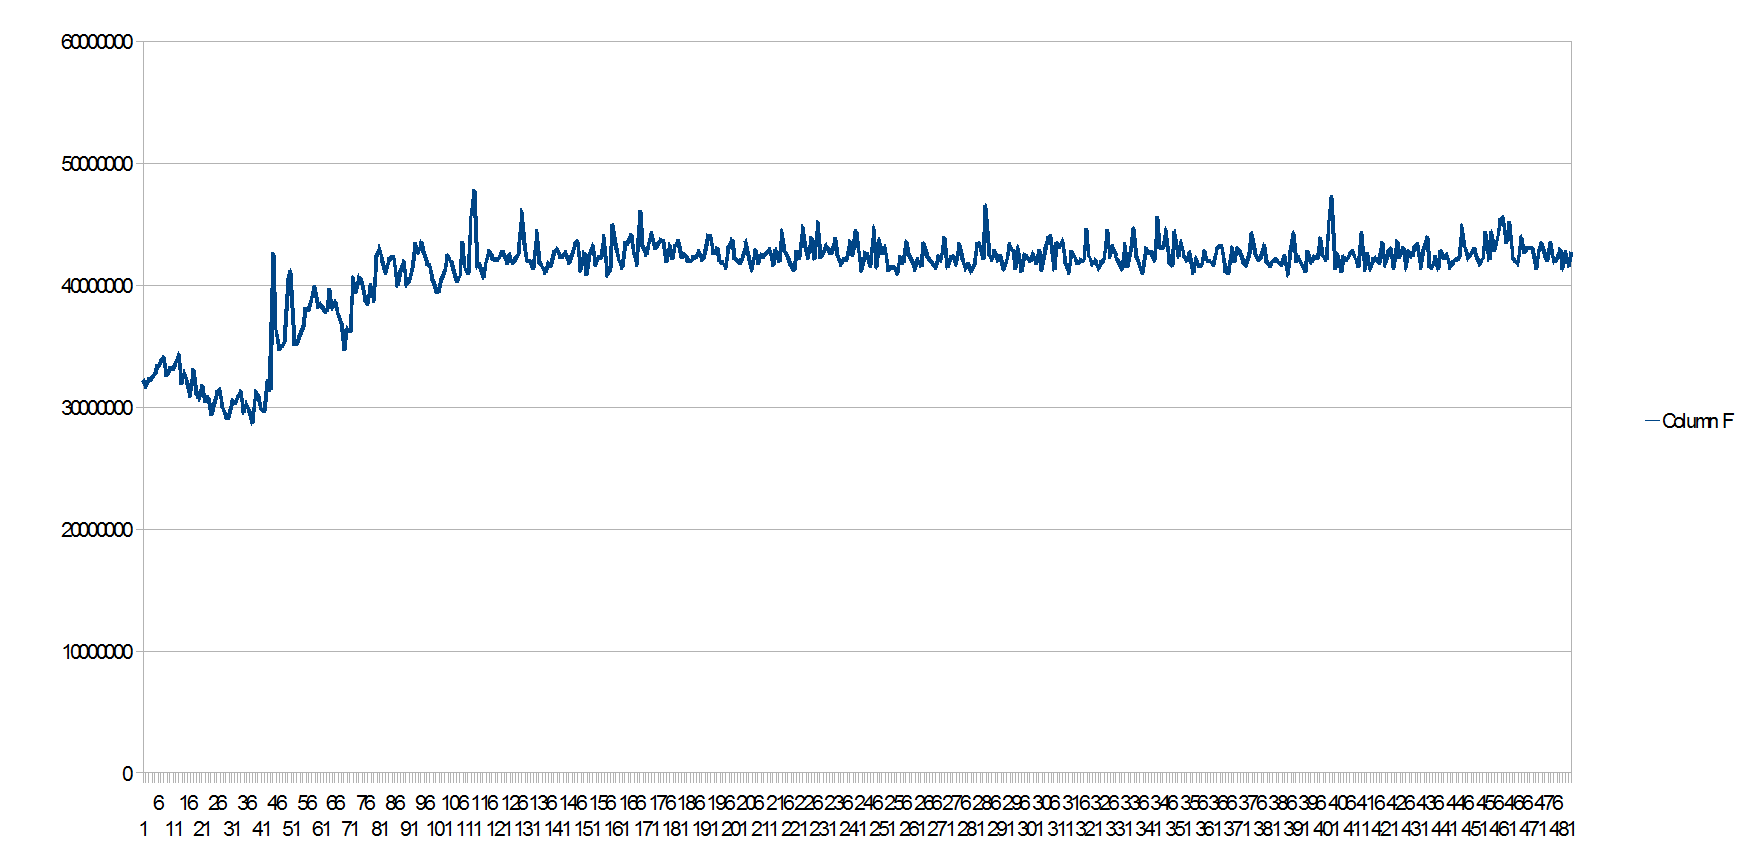
\includegraphics[width=1.00\textwidth]{Media/gpu_timer_hybrid.png}
	\caption{Output from GL TIME ELAPSED per frame for a hybrid scene. Time is averaging around 42.0 milliseconds.}	
	\label{fig:hybrid_gpu_time}
\end{figure}

\begin{figure}[H]
	\centering
	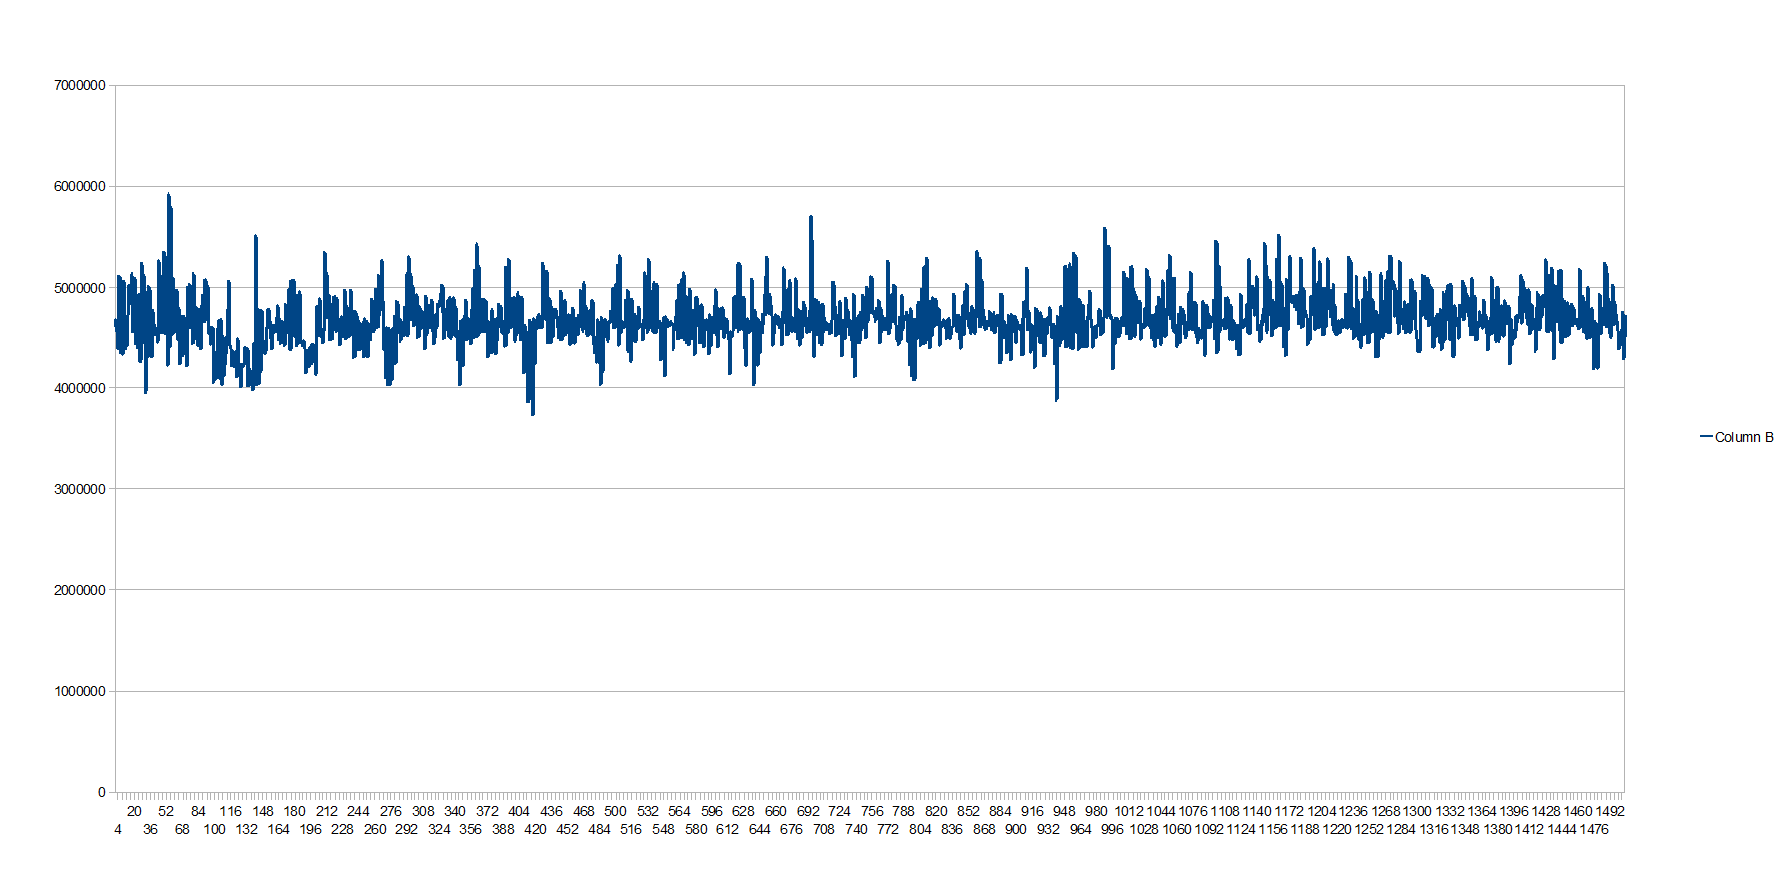
\includegraphics[width=1.00\textwidth]{Media/gpu_timer_raster_only.png}
	\caption{Output from GL TIME ELAPSED per frame for a purely rasterized scene. Time is averaging around 4.5 milliseconds.}
	\label{fig:raster_gpu_time}
\end{figure}

As figure \ref{fig:hybrid_gpu_time} and figure \ref{fig:raster_gpu_time} show, the hybrid scene is about ten times slower than the purely rasterized scene at a screen resolution of 1024x768.

\section{What went wrong}
In the end, the hybrid test configurations we managed to create were limited to raytracing the normals of the scene geometry and push that into the final deferred shading pass to use for lighting. We had a fully working raytraced shadows implementation in OptiX, but we couldn't get past some really bad crashes that was caused during interop, that just wouldn't allow us to move forward any further. Thus we never got to really test any hybrid configurations of true interest. But this was barely the icing on the cake of problems we encountered during the duration of our work.

The thesis was originally supposed to explore volume rendering with the OptiX raytracing framework, and how to combine that with a rasterized scene. We spent the good half of February 2012 researching volume rendering. We were thinking of exploring compositing volume graphics with typical solid-surface realtime graphics. Tile-based deferred rendering was of high interest to us, and we decided to study the ways this relatively new technique could be combined with realtime raytracing. Both deferred rendering with rasterization and raytracing are relatively old techniques that have recently become relevant for realtime graphics. Deferred pipelines became popular around 2004-2005 when GPUs finally had enough memory to allow multiple G-buffers to be held in memory. Raytracing on GPUs has become easy to program thanks to languages like OpenCL and CUDA. Since a deferred renderer outputs much of the information needed (surface position and normal) to start secondary rays, we thought combining the two could be advantageous.

We had an OpenGL based deferred renderer up and running fast, and the idea was to plug OptiX into this, as it seemingly had good interopability with OpenGL. Sadly, we spent a lot of time fighting crashes caused by OptiX and OpenGL interop. Having to wait for minutes to recover from display driver crashes sapped hours of development time, to the point where we were afraid this could damage our hardware. The retained-mode API-behaviour of OptiX hasn't helped when integrating it into our render-stage based framework either. OptiX isn't a bad library, it does what it claims very well, but it needs more users. For that to happen, it has to become more open and work on other vendors hardware. In hindsight, we should have written the raytracer ourselves.

Midway through the project, we decided we needed a scene that could showcase the properties of a hybrid. The BART project seemed like a perfect fit. One of the sample scenes contains mostly diffuse shaded geometry and some translucent geometry. It took some effort getting the BART parser into a workable state. The point of using BART was somewhat lost, as we didn't have time to implement the animation part of it, so, we couldn't compare our renderer against other implementations.

We didn't have a clear plan of distributing work between the rasterizer and the raytracer, this was supposed to be part of the experimentation of the thesis. Should only parts of the screen be raytraced? Should the raytracer handle soft omni-directional shadows? Should the rasterizer only handle its G-buffer creation, and OptiX the final shading? We tried to do too much. Much time was spent on details such as C++ design and architecture, and we greatly underestimated the effort it would take to get into the OptiX programming model.

\section{What went right}
We set out with a pretty solid engine architecture. Wrapping OpenGL functionality into object oriented code that would safely create and destruct itself, with simplified interfaces for interacting with the underlying OpenGL functionality worked really well.


\section{Further work}

The work presented in this thesis can be improved. 
\begin{itemize}
	\item We identified that graphics hardware drivers are still not handling interoperation between Cuda and OpenGL fast enough. Using OpenGL 4.3, a raytracer could be implemented in the Compute Shader stage, which should cancel the interoperation overhead.
	\item The deferred renderer could be rewritten to take advantage of tile-based parallellization in it's lighting pass. Using OpenGL 4.3, this could also be handled in a Compute Shader now, and probably also integrate well with a Compute Shader based raytracer.
	\item Improve the BART loader to support animations. That would allow us to compare performance with other BART renderers.
	\item Extend the raytracer with intersect programs for geometry that is better suited for raytracing than rasterization, like NURBS, Meta Shapes and Distance Fields.
\end{itemize}


\begin{thebibliography}{9}

%\bibitem{cite_mnemonic}
% Author(s)
% Paper title
% publisher
% edition
% year of publication

\bibitem{jensen95}
  Henrik Wann Jensen and Niels J�rgen Christensen
  "Photon maps in Bidirectional Monte Carlo Ray Tracing of Complex Objects"
  Computers and Graphics 19 (2), pp.215-224, 1995

\bibitem{joao10}
  Jo�o Cabeleira,
	"Combining Rasterization and Ray Tracing Techniques to Approximate Global Illumination in Real-Time"
  Instituto Superior T�cnico,
  www.voltaico.net
  2010
  
\bibitem{nv2012}
  Nvidia Corporation,
  "OptiX Ray Tracing Engine Programming Guide version 2.5"
  27. January 2012

\bibitem{Parker10OptiX}
  Parker et al.,
  "OptiX: A General Purpose Ray Tracing Engine"
  ACM 2010
  
\bibitem{Mania2008}
	K. Mania and E. Reinhard
	"Improving Interaction Performance for Ray Tracing"
	Eurographics Short Paper
	2008
\bibitem{dachsbacher2005}
  Carsten Dachsbacher and Marc Stamminger, 
  "Reflective Shadow Maps", 
  in Symposium on Interactive 3D Graphics , 
  New York, USA, 2005, 
  pp. 203 - 231.

\bibitem{mcguire2009}
  Morgan McGuire and David Luebke,
  "Hardware-Accelerated Global Illumination by Image Space Photon Mapping",
  Proceedings of the 2009 ACM SIGGRAPH/EuroGraphics conference on High   Performance Graphics,
  2009,
  http://graphics.cs.williams.edu/papers/PhotonHPG09/

\bibitem {kaplanyan2009}
  Anton Kaplanyan, "Light Propagation Volumes in CryEngine3", in Advances in Real-Time 
  Rendering in 3D Graphics and Games Course,
  SIGGRAPH, 
  2009

\bibitem {purcell2002}
Timoty Purcell, Ian Buck, William Mark, and Pat Hanrahan, 
"Ray Tracing on Programmable Graphics Hardware", 
International Conference on Computer Graphics and Interactive Techniques, 2002

\bibitem {popov2007}
Stefan Popov, Johannes G�nthe, Hans-Peter Seidel, and Philipp Slusallek, 
"Stackless KDTree Traversal for High Performance GPU Ray Tracing", 
Computer Graphics Forum, vol. 26, 
no. 3, pp. 415-424, September 2007.

\bibitem {crassin2011}
Cyril Crassin, Fabrice Neyret, Miguel Sainz, Simon Green, Elmar Eisemann
"Interactive Indirect Illumination Using Voxel Cone Tracing",
Pacific Graphics 2011

\bibitem {optixpage}
Optix. [Online]. http://www.nvidia.com/object/optix.html

\bibitem {reyes1987}
Cook, Carpenter, Catmull
"The Reyes Image Rendering Architecture"
Pixar

\bibitem {pixar_subdiv}
Pixar. [Online] http://graphics.pixar.com/opensubdiv

\bibitem {bart_homepage}
Jonas Lext, Ulf Assarsson, and Tomas M�ller 
[Online] http://www.ce.chalmers.se/BART/
Department of Computer Engineering, Chalmers University of Technology, Sweden. 

\end{thebibliography}

\end{document}
